\documentclass[border=12pt]{standalone}
% shared preamble for all schematics/diagrams
\usepackage[siunitx, RPvoltages, european resistors]{circuitikz}
\usepackage{tikz}
\usetikzlibrary{arrows.meta,positioning,calc,shapes.geometric,fit,backgrounds,decorations.pathreplacing}
\usepackage[scaled=0.92]{helvet}
\renewcommand{\familydefault}{\sfdefault}
\usepackage{xcolor}
\usepackage{amsmath}
\usepackage{ifthen}
\definecolor{ink}{HTML}{1F2328}
\definecolor{muted}{HTML}{6B6A66}
\definecolor{c1}{HTML}{2A78D6}
\definecolor{c2}{HTML}{EB6834}
\definecolor{c3}{HTML}{1BAF7A}
\definecolor{c4}{HTML}{6250D6}
\definecolor{fill1}{HTML}{EAF2FC}
\definecolor{fill2}{HTML}{FDEEE7}
\definecolor{fill3}{HTML}{E6F6EF}
\definecolor{fill4}{HTML}{EFEDFB}
\definecolor{hv}{HTML}{C62828}
\ctikzset{bipoles/thickness=1.2, monopoles/ground/thickness=1.2}
\tikzset{every picture/.style={line width=0.7pt, color=ink}}

\begin{document}
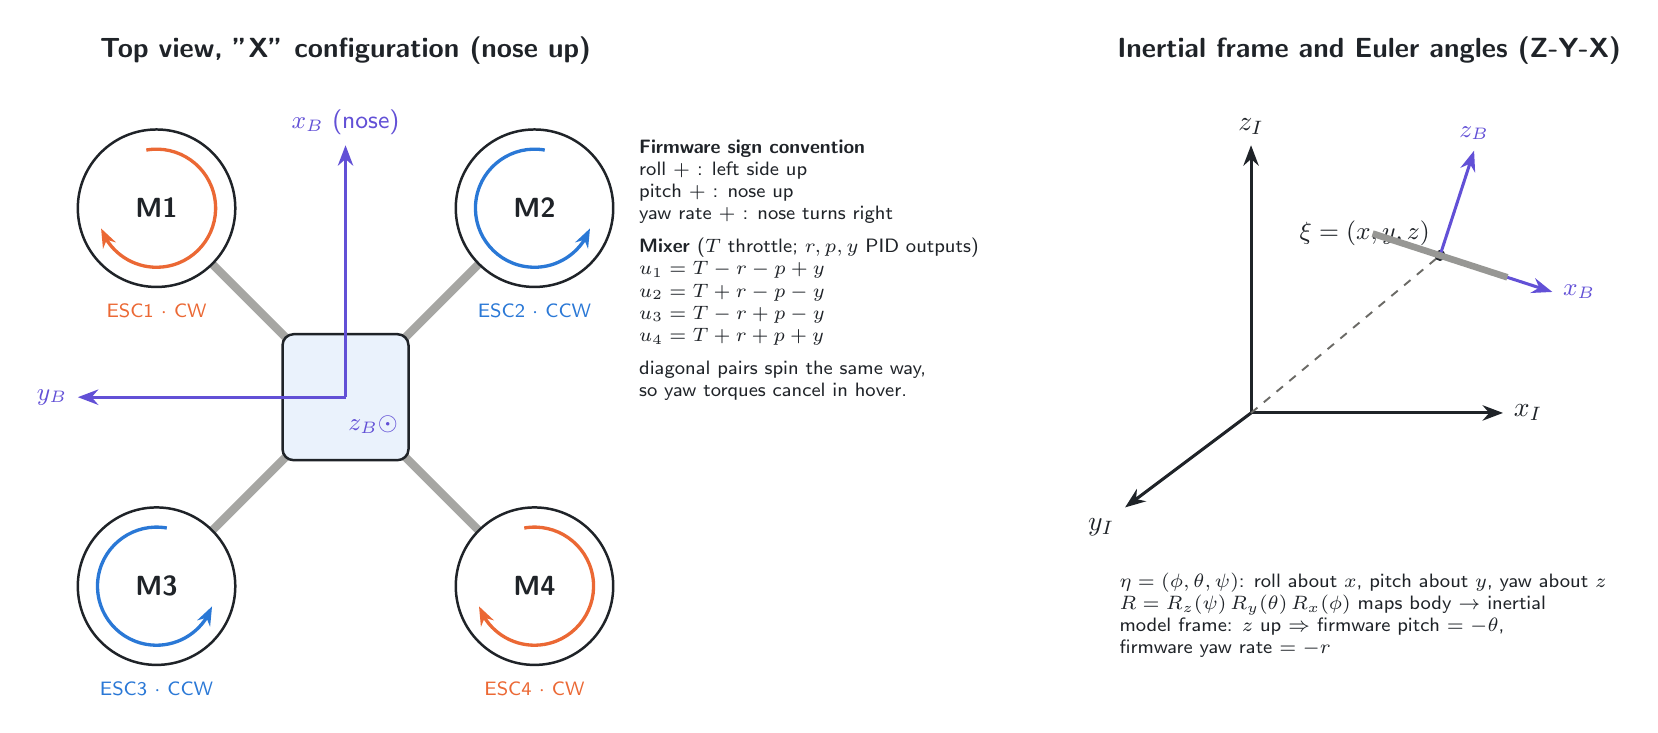
\begin{tikzpicture}[a/.style={line width=1.1pt, -{Stealth[length=2.6mm]}}]
% ---------------- top view ----------------
\node[font=\bfseries] at (0,4.4) {Top view, "X" configuration (nose up)};
\draw[line width=3pt, muted!60] (-2.4,2.4) -- (2.4,-2.4);
\draw[line width=3pt, muted!60] (-2.4,-2.4) -- (2.4,2.4);
\draw[fill=fill1, line width=0.9pt, rounded corners=4pt] (-0.8,-0.8) rectangle (0.8,0.8);
\foreach \x/\y/\n/\d/\c in {-2.4/2.4/1/CW/c2, 2.4/2.4/2/CCW/c1, -2.4/-2.4/3/CCW/c1, 2.4/-2.4/4/CW/c2} {
  \draw[fill=white, line width=0.9pt] (\x,\y) circle (1.0);
  \node[font=\bfseries] at (\x,\y) {M\n};
  \ifthenelse{\equal{\d}{CW}}
    {\draw[\c, line width=1.2pt, -{Stealth[length=2.4mm]}] ($(\x,\y)+(100:0.75)$) arc (100:-160:0.75);}
    {\draw[\c, line width=1.2pt, -{Stealth[length=2.4mm]}] ($(\x,\y)+(80:0.75)$) arc (80:340:0.75);}
  \node[font=\scriptsize, \c] at ($(\x,\y)+(0,-1.3)$) {ESC\n{} $\cdot$ \d};
}
% body axes
\draw[a, c4] (0,0) -- (0,3.2) node[above, font=\small] {$x_B$ (nose)};
\draw[a, c4] (0,0) -- (-3.4,0) node[left, font=\small] {$y_B$};
\node[c4, font=\small] at (0.35,-0.35) {$z_B\odot$};
\node[font=\scriptsize, align=left, anchor=north west] at (3.6,3.4) {
\textbf{Firmware sign convention}\\
roll $+$ : left side up\\
pitch $+$ : nose up\\
yaw rate $+$ : nose turns right\\[4pt]
\textbf{Mixer} ($T$ throttle; $r,p,y$ PID outputs)\\
$u_1 = T - r - p + y$\\
$u_2 = T + r - p - y$\\
$u_3 = T - r + p - y$\\
$u_4 = T + r + p + y$\\[4pt]
diagonal pairs spin the same way,\\so yaw torques cancel in hover.};

% ---------------- side view / inertial ----------------
\begin{scope}[xshift=11.5cm, yshift=-0.2cm]
\node[font=\bfseries] at (1.5,4.6) {Inertial frame and Euler angles (Z-Y-X)};
\draw[a, ink] (0,0) -- (3.2,0) node[right] {$x_I$};
\draw[a, ink] (0,0) -- (-1.6,-1.2) node[below left] {$y_I$};
\draw[a, ink] (0,0) -- (0,3.4) node[above] {$z_I$};
\draw[dashed, muted] (0,0) -- (2.4,2.0);
\fill (2.4,2.0) circle (2pt) node[above left, font=\small] {$\xi = (x, y, z)$};
\begin{scope}[shift={(2.4,2.0)}, rotate=-18]
  \draw[a, c4] (0,0) -- (1.5,0) node[right, font=\small] {$x_B$};
  \draw[a, c4] (0,0) -- (0,1.4) node[above, font=\small] {$z_B$};
  \draw[line width=2.4pt, muted!70] (-0.9,0) -- (0.9,0);
\end{scope}

\node[font=\scriptsize, align=left, anchor=north west] at (-1.8,-1.9) {
$\eta = (\phi,\theta,\psi)$: roll about $x$, pitch about $y$, yaw about $z$\\
$R = R_z(\psi)\,R_y(\theta)\,R_x(\phi)$ maps body $\to$ inertial\\
model frame: $z$ up $\Rightarrow$ firmware pitch $= -\theta$,\\ firmware yaw rate $= -r$};
\end{scope}
\end{tikzpicture}
\end{document}
